\subsection{Caso d'uso UC10: Creazione dell'infografica}
\begin{figure}[h] 
	\centering 
	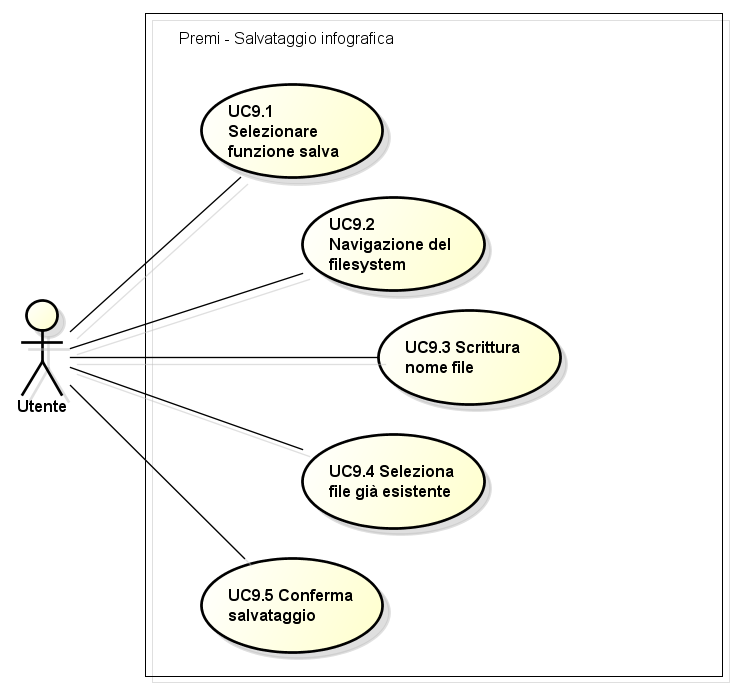
\includegraphics[scale=0.45] {img/UC10.png}
	\caption{UC10 - Creazione dell'infografica}
\end{figure}

\begin{itemize}
	\item \textbf{Attori:} Proprietario;
	\item \textbf{Scopo e descrizione:} L'utente ha creato una presentazione e da questa vuole creare un'\gls{infografica}. Con l'opportuno tool può scegliere il \gls{template} da usare e le \gls{slide} da includere in essa. Una volta completata la procedura verrà creata l'\gls{infografica} corrispondente in modo automatico, prendendo le informazioni contenute nelle \gls{slide} scelte e disponendole a seconda del \gls{template} scelto;
	\item \textbf{Precondizione:} L'utente ha creato una nuova presentazione nella fase di creazione di un progetto o ha aperto un progetto creato in precedenza e ha selezionato il comando per creare l'\gls{infografica} della presentazione;
	
	\item \textbf{Flusso principale degli eventi:}
	\begin{enumerate}
		\item L'utente sceglie un \gls{template} [UC10.1];
		\item L'utente sceglie le \gls{slide} da inserire nell'\gls{infografica} [UC10.2];
		\item L'utente conferma la creazione dell'\gls{infografica} [UC10.3].
	\end{enumerate}
	\item \textbf{Postcondizione:} Il sistema ha creato l'\gls{infografica} a seconda delle scelte dell'utente.
\end{itemize}


\subsection{Caso d'uso UC10.1: Scegliere un template}
\begin{itemize}
	\item \textbf{Attori:} Proprietario;
	\item \textbf{Scopo e descrizione:} L'utente sceglie il \gls{template} con cui creare l'\gls{infografica};
	\item \textbf{Precondizione:} Il sistema ha aperto la finestra di dialogo per la scelta del \gls{template};
	\item \textbf{Postcondizione:} Il sistema registra la scelta del \gls{template} fatta dall'utente.
\end{itemize}


\subsection{Caso d'uso UC10.2: Scegliere le slide}
\begin{itemize}
\item \textbf{Attori:} Proprietario;
\item \textbf{Scopo e descrizione:} L'utente sceglie quali \gls{slide} del suo progetto inserire nell'\gls{infografica};
\item \textbf{Precondizione:} L'utente ha scelto il \gls{template} con cui creare l'\gls{infografica};
\item \textbf{Postcondizione:} Il sistema registra la scelta delle \gls{slide} fatta dall'utente.
\end{itemize}


\subsection{Caso d'uso UC10.3: Conferma della creazione dell'infografica}
\begin{itemize}
\item \textbf{Attori:} Proprietario;
\item \textbf{Scopo e descrizione:} L'utente vuole confermare la creazione dell'\gls{infografica};
\item \textbf{Precondizione:} L'utente ha scelto il \gls{template} e le \gls{slide} con cui creare l'\gls{infografica};
\item \textbf{Postcondizione:} Il sistema ha creato l'\gls{infografica}.
\end{itemize}

